%!TEX root = ../../thesis.tex

%=============================================================================


\section{Orchestrator}
\label{main:orc}
In this section we will discuss the Orchestrator as part of the proposed framework.
The Orchestrator has to fulfill two major tasks, synchronizing results and determining the formats used to transmit audio, as discussed in the previous chapter \ref{main:lib:format_chooosing}.

First we will discuss the determination of audio in- \& output formats used internally by the library.
To achieve this, a number of factors have to be considered.
To reduce network traffic and improve transmission speed it is advantageous to transmit audio with the lowest possible bandwidth.
Consider two nodes, where one node transmits and one node receives audio which differs only in that one node internally works with 16kHz and the other with 48kHz.
In this scenario, resampling should happen at the node which works with 48kHz, in order to transmit only 16kHz audio.

However, it may be the case that network capacity is abundant while CPU capacity is not, e.g. in embedded systems.
Consider a node outputting an audio signal at 16kHz, and four nodes requiring this audio signal at 48kHz, e.g. a \gls{vad}, gender-, emotion-, and voice recognition.
In this scenario, one may opt to not resample four times, but rather once and transmit the higher bandwidth audio, or, more generally speaking, minimize the number of resamplings happening in the pipeline.

To tackle this issue, we developed two algorithms which could each handle one of these cases and added a simple way to add new algorithms, should the need arise.
The first algorithm introduces a cost function which calculates the bandwidth of each topics formats.
This algorithm is formalized in figure \ref{main:orc:resampling:formula:min_traffic}.
It applies the aforementioned cost function $cost_{format}$ on each in- \& output format for a given topic and then chooses the minimum as the optimal.

\begin{figure}
	\begin{align}
	cost_{format} &= channel\_count \cdot bitrate_{signal} \cdot frequency\\
	format_{optimal} &= min({bitrate_{i}\ |\ i \in formats_{input} \cup formats_{output}})
	\end{align}
	\caption{Formula to calculate the lowest bandwidth format out of a given set of in- \& output formats.
		The $bitrate_{signal}$ is the amount of bits a single sample requires, while the $bitrate_{i}$ is the $cost_{format}$ of the format $i$.}
	\label{main:orc:resampling:formula:min_traffic}
\end{figure}

The second algorithm is a bit more complex, as it prioritizes the amount of resamplings over the used bandwidth when choosing the right format.
It is formalized in figure \ref{main:orc:resampling:formula:min_cpu}.
As such, it calculates for each format on a given topic the number of resamplings that would occur, if that format was chosen for this topic.
Then the format which has the fewest resamplings is chosen as the optimal format.
However, there may be several formats which fulfill this condition.
If this is the case, it comes naturally to mind to choose the format which requires the least amount of bandwidth, so the algorithm formalized in figure \ref{main:orc:resampling:formula:min_traffic} is used to choose the optimal format of the formats which require the least amount of resampling.

\begin{figure}
	\begin{align}
	\alpha(i,k) &=
	\begin{cases}
	1 & , i = k \\
	0 & , i \neq k
	\end{cases} \\[10pt]
	resamplings_{format} &= \sum_{f=1}^{F} \alpha(format, f) ,\ f \in formats\\[10pt]
	format_{optimal} &= argmin_{f}(resamplings_{f}) , \ f \in formats
	\end{align}
	\caption{Formula to calculate the lowest bandwidth format out of a given set of in- \& output formats.
		The $bitrate_{signal}$ is the amount of bits a single sample requires, while the $bitrate_{format}$ indicates, how many bits a second of this signal require.}
	\label{main:orc:resampling:formula:min_cpu}
\end{figure}

After the Orchestrator determined the transmission format for each topic, it will inform all registered components about their respective internally used audio formats via a \gls{ros}-message.
The library part of each component will listen to these messages and then store and use these formats as discussed in chapter \ref{main:lib:format_chooosing}.
It is important to note at which points in time the Orchestrator will determine the audio formats.
Since it cannot conclusively determine if all components that are going to be started have already registered, as it lacks a list of such components, whenever a component registers the formats of all topics are determined anew.
Additionally, a component may die or shut down at any point in time.
When this is detected, all formats are determined as well, since the Orchestrator cannot foretell how long the pipeline will still run in the current configuration and more profitable audio formats may save a lot of bandwidth or computation time, or improve the quality of the transmission, by not unnecessarily resampling and converting audio.  

Determining whether a component has shut down must be conducted by the Orchestrator.
For this reason it will routinely ping all components via \gls{ros} inbuild \gls{ros}-node pinging functionality.
Should \gls{ros} not find a node in question, or should the node be non-responding, the Orchestrator will remove it from its internally kept list of active nodes and terminate all communication with it.
Such nodes will furthermore not be considered for fusion of results anymore. 

\subsubsection{Result Fusion}

When synchronizing results, a few key circumstances need to be kept in mind.
The first and probably most important one is that because of our library and the relentless efforts to annotate our audio and in turn results with timestamps, the synchronization of the results itself is rather trivial.
There are however still a few possible pitfalls.
Most importantly, the Orchestrator can not know with certainty when results are arriving, or -more precisely- when all of the results to be synchronized will have arrived.
This is rather unfortunate, as it is of utmost importance to relay all information as soon as possible, to keep further programs reliant on our synchronized results, such as natural language processors or robot behavior controllers, not waiting and thus keep latency down to a minimum.
There is another important question we have evaded up until now.
When we synchronize our results,with respect to what do we synchronize?
After all, results of different types may overlap within the time frame of their respective occurrence.
An example of this phenomenon can be observed in figure \ref{pic:main:orc:result_overlap}.
The first result of an \gls{asr} node, A1, may be fused with the first result of an \gls{ssl} node, S1.
This however occurred partially with A2, which may be also fused for our result.
This could iteratively go on until all shown results may be fused together.
This is naturally not desirable, as the latency of the first results would needlessly increase and no meaningful information could be gained by this synchronization.

\begin{figure}[]
	\centering
	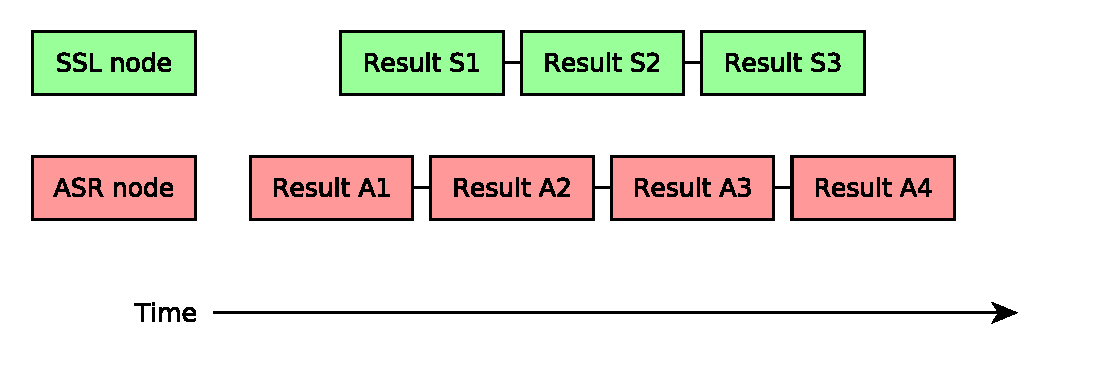
\includegraphics[width=\textwidth]{diagrams/main_orc_result_overlap.pdf}
	\caption{Overlap of results from two distinct components, an \gls{ssl} component in green and an \gls{asr} component in red.
		Trying to synchronize as much results as possible may result in a macro result containing all presented data.}
	\label{pic:main:orc:result_overlap}
\end{figure}


A few approaches to deal with this problem may come to mind.
We could for example choose to synchronize with respect to each recorded audio message.
But due to the library not enforcing a singular, constant size for the audio transmitted via these messages (see chapter \ref{main:lib:augmented_audio_msg} and chapter \ref{basics:latency} for the reasoning), this could quickly explode in complexity; especially since a beamformer may create a new artificial audio signal which may either transport smaller audio signals with each message or slightly shift the timestamps of the messages, due to factoring in the time-of-arrival differences for the different microphones.
This way, all -or worse, just some- of the results may have been computed on timestamps differing from the originally recorded ones.

The approach we ultimately chose was to determine one so called anchor type, which would then be the basis of all synchronization.
Each result received of this anchor type would by their timestamps determine the timeframe with which all results of other types would then be synchronized with.
Any result occurring at least partially in this timeframe would be included in the fused result.

Initially we planned to only use speech utterances as anchor.
However, as time moved on, we realized that this may not be the only interesting type for synchronization.
Programs for tracking persons for example could be very interested in obtaining data on which particular person was speaking at a given moment, synchronized with their position provided by \gls{ssl} information.
And so our algorithms would quickly be adapted to not only use every result type as anchor type, but to do so concurrently.
This puts us in the favorable position to provide any result type of particular interest without giving up synchronization with other results.

- actual 

For each anchor result the Orchestrator receives, it creates a new meta fusion object

%-------------------------


The most important task of the Orchestrator is to gather the information almost every node of the pipeline produces, fuse them and then provide these fused information.
There are a number of factors to consider when designing a solution for this task.
\begin{enumerate}
	\item How to actually synchronize?
	\item How to handle missing information or information which take a long time to compute?
	\item third thing
\end{enumerate}

Second, it needs to synchronize the nodes results and output them. 
%-------------------------

Algorithms

- algo zur synchronisierung der ergebnisse 

- einfach nur relativ großer timeout?

- zusätzlich heuristik über die bisher benötigten zeiten


\begin{itemize}
	\item manages all participating nodes
	\item determines used audio formats for transmission
	\item handles synchronization task
	\item handles meta data accumulation, introspection and acts on anomalies
\end{itemize}

meta information gathering:

\begin{itemize}
	\item how the orchestrator gathers meta information and what exactly he gathers
	\item how this information is then used
\end{itemize}

algorithms implemented for the orchestrator

\begin{itemize}
	\item minimizing amount of resampling
	\item how is synchronization/ fusion solved?
	\item feedback to user if a non-optimal configuration is found (algorithm on how to find those)
\end{itemize}

\subsection{Meta Information Gathering}
It is desirable to gather meta information about results delivered by nodes. 
I.e. probability of a certain result and time to compute. 
Time to compute can be used to better predict if a node will deliver a result at all. 
See synchronization of results in the orchestrator algorithms chapter.

Method 1: Every results need to be enhanced with meta informations

pro

- relatively easy to implement

con

-nodes need to explicitly keep track on this information and fill them (user unfriendly)

- results bigger than they need to be

- Method 2: TTC can be computed by orchestrator, other meta information included 

pro

-TTC can be expected to always exist and be correct (can not be expected if nodes are expected to calculate it)

-node implementation is not blown up

con

-not all nodes provide results, so beamformer and filter nodes need to provide the meta information explicitly

-how would this work?

-each result message has a timestamp, in combination with the audio flow graph calculated by the orchestrator, the time from one result to the next in line is roughly the time the next node took for computation


\subsection{Fusion}
- One of the if the most important tasks of the Orchestrator is the fusion of each components results.

- For each registered component

- This allows the Orchestrator to adapt the maximum time it waits for each component on the fly, while running.

- Due to the Orchestrator saving all incoming results with their respective latency to a database, it is also possible to load the database of a previous run.

- 


\begin{figure}
	\begin{align}
	latency_{fusion} = V_A \cdot max(\{\frac{1}{n_i} \cdot \sum_{k=1}^{n_i} l_{i,k}\ | \ i \in components\})
	\end{align}
	\caption{Maximum latency of a single fusion.
		$V_A$ is a constant, typically 1.5.
		$n_i$ is the amount of results the orchestrator already received of a component $i$.
		$l_{i,k}$ is the latency of the $k$th result of the component $i$.}
	\label{main:orc:latency:formula}
\end{figure}